\section{Interface Gráfica do \textit{Boilerplate}}
\label{sec:3:interface-grafica}

Além de todos os componentes e abstrações apresentados, a interface gráfica é um dos principais elementos do \textit{boilerplate}. A interface foi desenvolvida utilizando a biblioteca \texttt{PyGObject}, que fornece uma API para a criação de interfaces gráficas em Python. A seguir, são apresentadas as principais características e funcionalidades da interface gráfica do \textit{boilerplate} ilustradas na Figura~\ref{fig:3:gui}.

\begin{figure}[h!]
    \centerline{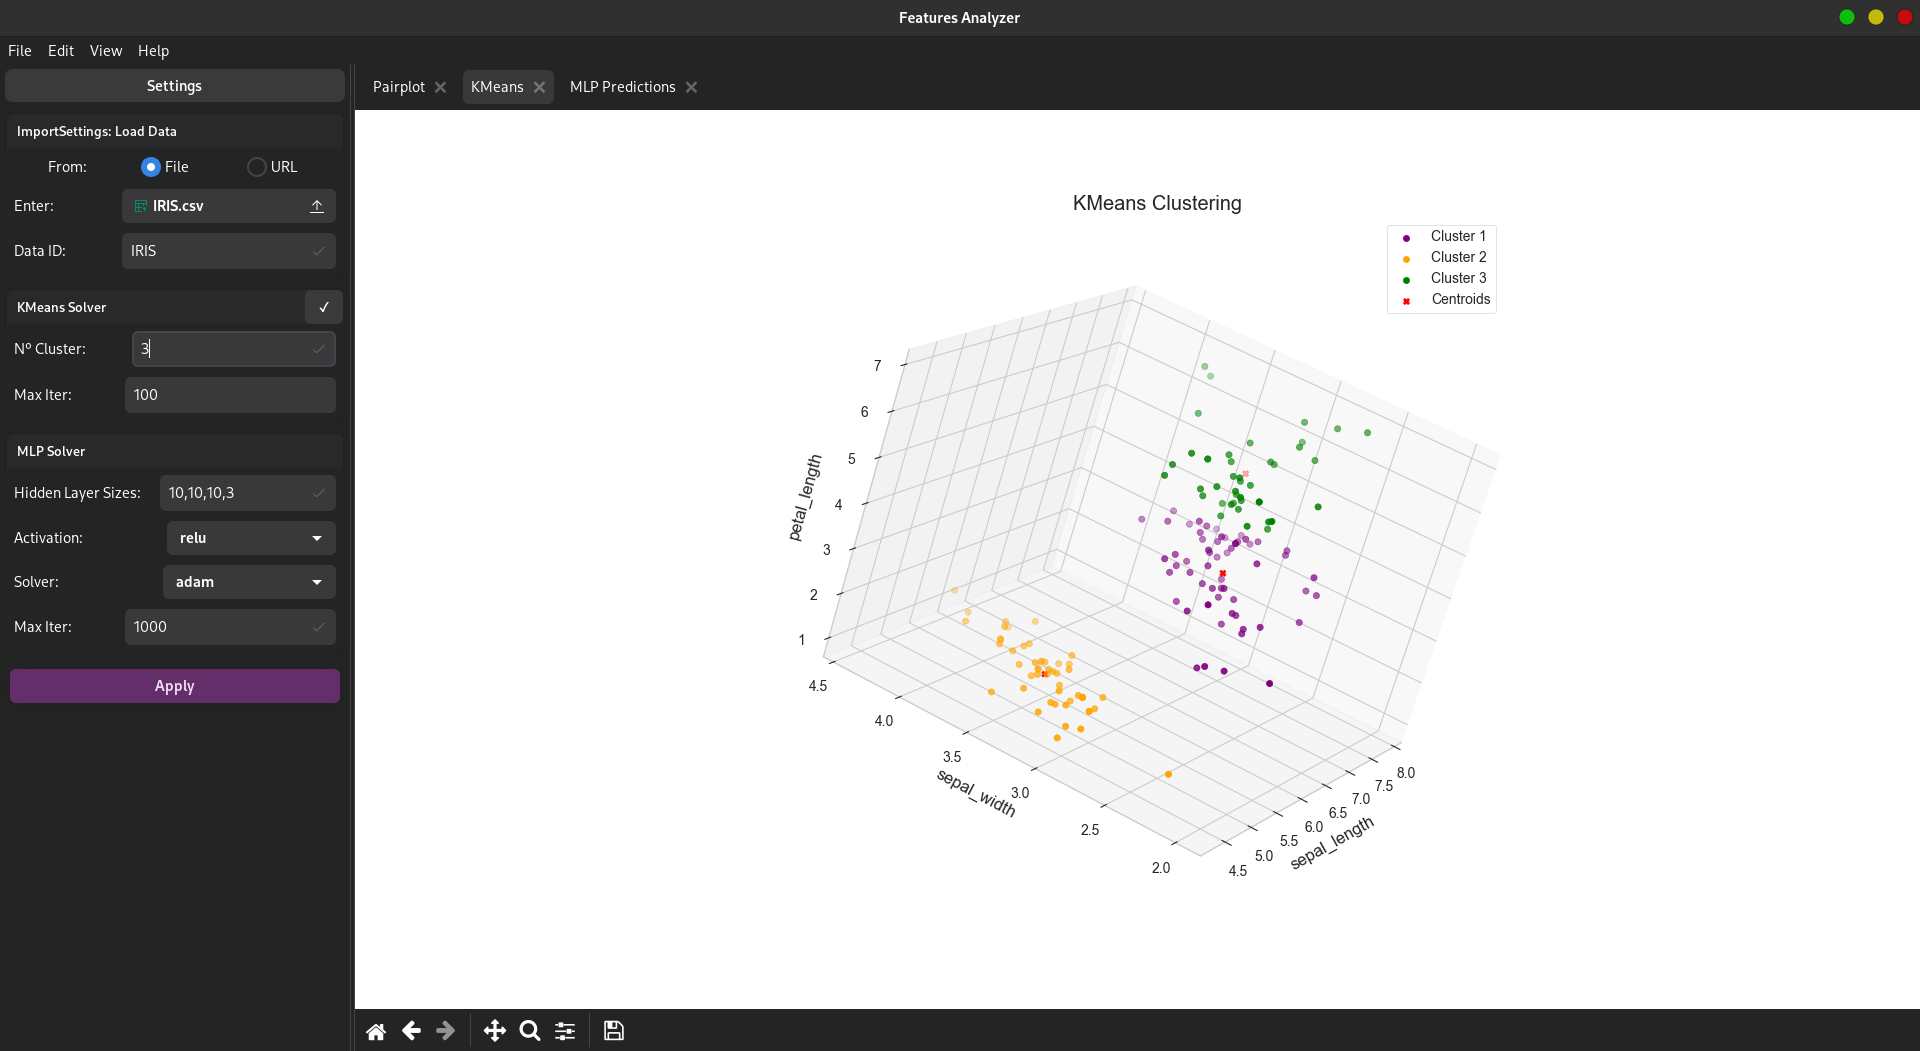
\includegraphics[width=0.8\columnwidth]{image/source/gui.png}}
    \caption{Interface Gráfica do \textit{Boilerplate}}
    \centerline{\textbf{Fonte:} O Próprio Autor (2025)}
    \label{fig:3:gui}
\end{figure}

\begin{itemize}
    \item \textbf{Barra de Ferramentas}: Localizada na parte superior da janela, a barra de ferramentas contém botões para ações comuns, como abrir, salvar e executar, além de menus para configurações e ajuda. Esse componente deve ser ajustado para atender às necessidades específicas de cada aplicação.
    \item \textbf{Barra Lateral} (\textit{sidebar}): À esquerda da janela, a barra lateral exibe os componentes disponíveis para interação, como configurações de importação e parâmetros de modelos. A responsabilidade pela importação dos dados para a memória é gerenciada pela biblioteca \texttt{Pandas}.
    \item \textbf{Área de Trabalho}: O espaço central da janela é dedicado à exibição de gráficos. O componente consiste em um \textit{widget} de \texttt{Gtk.Notebook} que permite alternar entre diferentes visualizações.
\end{itemize}

A interface gráfica é completamente customizável e extensível, permitindo a adição de novos componentes, personalização de estilos e integração com outras bibliotecas gráficas.

A arquitetura do \textit{boilerplate} facilita a criação de interfaces intuitivas e eficientes, oferecendo como exemplo a implementação do \texttt{KMeans} e \texttt{MLP} (\textit{Multi-Layer Perceptron} ou Perceptron de Múltiplas Camadas) para tratar o famoso conjunto de dados flor Iris.